%% Hand-authored TikZ schematic for the Method section: the two-layer terrain
%% geometry and the three fade functions over the same transition budget.
\begin{figure}[htb]
\centering
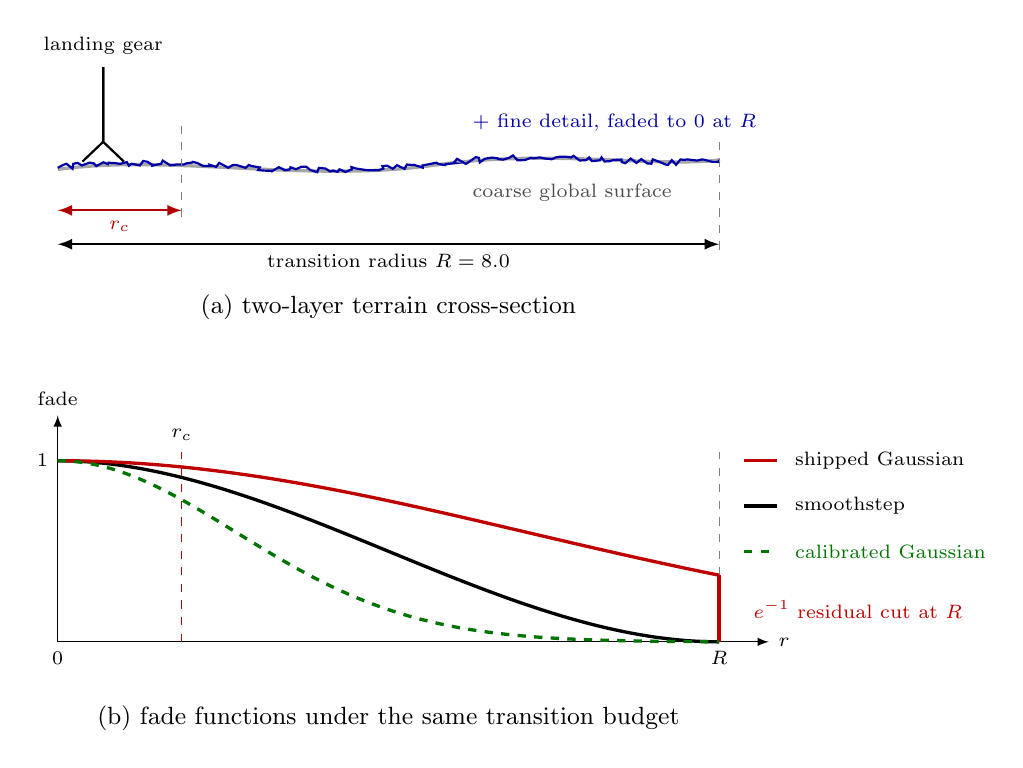
\begin{tikzpicture}[x=1.05cm, y=1cm, >=latex, font=\small]

%% ---- panel (a): two-layer cross-section --------------------------------
\begin{scope}
  % coarse global surface
  \draw[very thick, gray!70]
    (0,0) .. controls (1.4,0.20) and (3.0,-0.18) .. (4.6,0.06)
          .. controls (6.0,0.26) and (7.2,0.02) .. (8.0,0.12);
  % fine detail riding on it, faded out by R
  \draw[thick, blue!65!black, decorate,
        decoration={random steps, segment length=1.6pt, amplitude=1.1pt}]
    (0,0.02) .. controls (1.4,0.22) and (3.0,-0.16) .. (4.6,0.07)
             .. controls (6.0,0.26) and (7.2,0.02) .. (8.0,0.12);

  % landing gear feet inside the contact footprint
  \draw[thick] (0.55,1.30) -- (0.55,0.35) -- (0.30,0.10);
  \draw[thick] (0.55,1.30) -- (0.55,0.35) -- (0.80,0.10);
  \node[font=\scriptsize, anchor=south] at (0.55,1.34) {landing gear};

  % radii
  \draw[<->, thick] (0,-0.95) -- (8.0,-0.95)
    node[midway, below, font=\scriptsize] {transition radius $R=\SI{8.0}{\metre}$};
  \draw[<->, thick, red!70!black] (0,-0.52) -- (1.5,-0.52)
    node[midway, below, font=\scriptsize] {$r_c$};
  \draw[dashed, gray] (1.5,-0.60) -- (1.5,0.55);
  \draw[dashed, gray] (8.0,-1.02) -- (8.0,0.45);

  \node[anchor=west, font=\scriptsize, gray!60!black] at (4.9,-0.30)
    {coarse global surface};
  \node[anchor=west, font=\scriptsize, blue!65!black] at (4.9,0.60)
    {$+$ fine detail, faded to $0$ at $R$};
  \node[font=\small] at (4.0,-1.75) {(a) two-layer terrain cross-section};
\end{scope}

%% ---- panel (b): the three fade functions --------------------------------
\begin{scope}[yshift=-6.0cm, x=1.05cm, y=2.3cm]
  \draw[->] (0,0) -- (8.6,0) node[right, font=\scriptsize] {$r$};
  \draw[->] (0,0) -- (0,1.25) node[above, font=\scriptsize] {fade};
  \node[below, font=\scriptsize] at (0,0) {$0$};
  \node[below, font=\scriptsize] at (8.0,0) {$R$};
  \node[left, font=\scriptsize] at (0,1) {$1$};
  \draw[dashed, gray] (8.0,0) -- (8.0,1.05);

  % smoothstep: t^2(3-2t), t = 1 - r/R  -- compact support, exactly 0 at R
  \draw[very thick, black, domain=0:8, samples=90, smooth]
    plot (\x, {(1-\x/8)*(1-\x/8)*(3-2*(1-\x/8))});
  % as-shipped Gaussian k=1: never reaches 0, hard-truncated at R
  \draw[very thick, red!75!black, domain=0:8, samples=90, smooth]
    plot (\x, {exp(-1*(\x/8)^2)});
  \draw[red!75!black, very thick] (8.0,0.368) -- (8.0,0);
  % calibrated Gaussian k = ln 1000
  \draw[very thick, green!45!black, dashed, domain=0:8, samples=90, smooth]
    plot (\x, {exp(-6.9078*(\x/8)^2)});

  % contact footprint band
  \draw[red!70!black, dashed] (1.5,0) -- (1.5,1.05);
  \node[font=\scriptsize, anchor=south] at (1.5,1.06) {$r_c$};

  % curve labels live in a key to the right of the plot, clear of every curve
  \node[font=\scriptsize, red!75!black, anchor=west] at (8.3,0.18)
    {$e^{-1}$ residual cut at $R$};
  \draw[very thick, red!75!black] (8.3,1.00) -- (8.7,1.00);
  \node[font=\scriptsize, anchor=west] at (8.8,1.00) {shipped Gaussian};
  \draw[very thick, black] (8.3,0.75) -- (8.7,0.75);
  \node[font=\scriptsize, anchor=west] at (8.8,0.75) {smoothstep};
  \draw[very thick, green!45!black, dashed] (8.3,0.50) -- (8.7,0.50);
  \node[font=\scriptsize, anchor=west, green!45!black] at (8.8,0.50) {calibrated Gaussian};
  \node[font=\small] at (4.0,-0.42)
    {(b) fade functions under the same transition budget};
\end{scope}

\end{tikzpicture}
\caption{Geometry of the blending problem. (a) The fine-detail local patch is
faded into the coarse global surface inside a fixed transition radius $R$; the
landing gear contacts the surface within the much smaller footprint radius
$r_c$. (b) The three candidate fade functions on the same budget. Smoothstep
has compact support and reaches exactly zero at $R$; the as-shipped Gaussian
($k=1$) still carries roughly $e^{-1}\approx\SI{37}{\percent}$ of its amplitude
at $R$, so hard truncation there leaves the seam this study measures; the
calibrated Gaussian ($k=\ln 1000$) decays to about one part in a thousand by
$R$. The hybrid follows the Gaussian inside $r_c$ and smoothstep beyond it, and
is analytically identical to smoothstep at the boundary}
\label{fig:geometry}
\end{figure}
